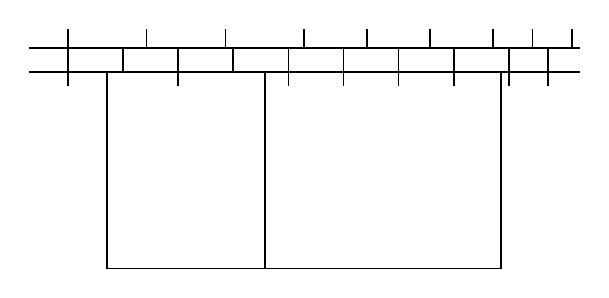
\begin{tikzpicture}[x=1cm,y=1cm,font=\normalsize,
 geometry edge/.style={solid,line width=.6pt},
 geometry mark/.style={solid,line width=.6pt},
 geometry label/.style={font=\normalsize,inner sep=2pt}]
\coordinate (W1) at (0,2.8);
\coordinate (W2) at (7,2.8);
\coordinate (W3) at (0,2.5);
\coordinate (W4) at (7,2.5);
\coordinate (R1) at (1,2.5);
\coordinate (R2) at (3,2.5);
\coordinate (R3) at (6,2.5);
\coordinate (R4) at (1,0);
\coordinate (R5) at (3,0);
\coordinate (R6) at (6,0);
\draw[geometry edge] (W1)--(W2);
\draw[geometry edge] (W3)--(W4);
\draw[geometry edge] (R1)--(R4);
\draw[geometry edge] (R2)--(R5);
\draw[geometry edge] (R3)--(R6);
\draw[geometry edge] (R4)--(R5);
\draw[geometry edge] (R5)--(R6);
\draw[geometry mark] (0.5,2.5)--(0.5,2.8);
\draw[geometry mark] (1.2,2.5)--(1.2,2.8);
\draw[geometry mark] (1.9,2.5)--(1.9,2.8);
\draw[geometry mark] (2.6,2.5)--(2.6,2.8);
\draw[geometry mark] (3.3,2.5)--(3.3,2.8);
\draw[geometry mark] (4.0,2.5)--(4.0,2.8);
\draw[geometry mark] (4.7,2.5)--(4.7,2.8);
\draw[geometry mark] (5.4,2.5)--(5.4,2.8);
\draw[geometry mark] (6.1,2.5)--(6.1,2.8);
\draw[geometry mark] (6.6,2.5)--(6.6,2.8);
\draw[geometry mark] (0.5,2.8)--(0.5,3.05);
\draw[geometry mark] (1.5,2.8)--(1.5,3.05);
\draw[geometry mark] (2.5,2.8)--(2.5,3.05);
\draw[geometry mark] (3.5,2.8)--(3.5,3.05);
\draw[geometry mark] (4.3,2.8)--(4.3,3.05);
\draw[geometry mark] (5.1,2.8)--(5.1,3.05);
\draw[geometry mark] (5.9,2.8)--(5.9,3.05);
\draw[geometry mark] (6.4,2.8)--(6.4,3.05);
\draw[geometry mark] (6.9,2.8)--(6.9,3.05);
\draw[geometry mark] (0.5,2.5)--(0.5,2.32);
\draw[geometry mark] (1.9,2.5)--(1.9,2.32);
\draw[geometry mark] (3.3,2.5)--(3.3,2.32);
\draw[geometry mark] (4.0,2.5)--(4.0,2.32);
\draw[geometry mark] (4.7,2.5)--(4.7,2.32);
\draw[geometry mark] (5.4,2.5)--(5.4,2.32);
\draw[geometry mark] (6.1,2.5)--(6.1,2.32);
\draw[geometry mark] (6.6,2.5)--(6.6,2.32);
\end{tikzpicture}